\documentclass{article}
\usepackage{arxiv}
%\documentclass[12pt]{article}
%\usepackage[cp1251]{inputenc}
%\usepackage[russian]{babel}

\usepackage[utf8]{inputenc}
\usepackage[english, russian]{babel}
\usepackage[T2A, T1]{fontenc}
\usepackage{url}
\usepackage{booktabs}
\usepackage{amsfonts}
\usepackage{nicefrac}
\usepackage{microtype}
\usepackage{lipsum}
\usepackage{comment}
\usepackage{graphicx}
\usepackage{natbib}
\usepackage{doi}
\usepackage{hyperref}
\usepackage{amssymb, amsmath, latexsym}
% \usepackage{fullpage}
\usepackage{algorithm}
\usepackage{algorithmic}
%\usepackage{algpseudocode}
\usepackage{tabularx}
\usepackage{paralist}
\usepackage{mathtools}
%\usepackage{tcolorbox}
\usepackage{xcolor}
\usepackage{amsmath}
\DeclareMathOperator*{\argmax}{arg\,max}
\DeclareMathOperator*{\argmin}{arg\,min}
\usepackage{algorithm}
\usepackage{algorithmic}
\usepackage{bbm} %for indicators 1
\usepackage{algpseudocode}
\usepackage{algorithm}
\usepackage{makecell}
\usepackage{multirow}
\usepackage{booktabs}
\usepackage{caption}
\usepackage{subcaption}
\usepackage{ dsfont }
\usepackage{nicefrac}  
\usepackage{hyperref}
\usepackage{subcaption}
% \usepackage{subfigure} 
\newcommand{\Exp}{\mathbf{E}}
\newcommand{\Prob}{\mathds{P}}
\newcommand{\R}{\mathbb{R}}
\newcommand{\E}{\mathbb{E}}
\newcommand{\e}{\varepsilon}
\newcommand{\eqdef}{\stackrel{\text{def}}{=}}

\newtheorem{theorem}{Theorem}
\newtheorem{Def}{Определение}[section]
\newtheorem{proposition}{Предположение}

\title{Сходимость с оценкой вероятностей больших отклонений для задач выпуклой оптимизации и седловых задач в условиях повышенной гладкости
}

\author{
	Рубцов Д.Н. \\
	\texttt{rubtsov.dn@phystech.edu} \\
	\And
	Гасников А.В. \\
	\texttt{gasnikov@yandex.ru} \\
}
\date{}

\renewcommand{\shorttitle}{Сходимость с оценкой вероятностей больших отклонений для задач выпуклой оптимизации и седловых задач в условиях повышенной гладкости}
\renewcommand{\undertitle}{}
%%% Add PDF metadata to help others organize their library
%%% Once the PDF is generated, you can check the metadata with
%%% $ pdfinfo template.pdf
\hypersetup{
pdftitle={Сходимость с оценкой вероятностей больших отклонений для задач выпуклой оптимизации и седловых задач в условиях повышенной гладкости},
pdfsubject={Сходимость с оценкой вероятностей больших отклонений для задач выпуклой оптимизации и седловых задач в условиях повышенной гладкости},
pdfauthor={Рубцов Д.Н., Гасников А.В.},
pdfkeywords={},
}

\begin{document}
\maketitle

\begin{abstract}
Классические результаты стохастической оптимизации, как правило, формулируются в терминах числа итераций, необходимых для достижения $\varepsilon$-точности по математическому ожиданию функции. В данной работе разрабатывается алгоритм, обеспечивающий гарантию сходимости с высокой вероятностью, причем предположения о "легкости хвостов" распределения шума стохастического градиента здесь не делаются, то есть  Минимизируемая функция здесь предполагается обладающей повышеннной гладкостью.

\end{abstract}


\keywords{: выпуклая оптимизация, седловые задачи, стохастическая оптимизация, тяжелые хвосты, повышенная гладкость, безградиентная оптимизация,  
}

\section{Введение}

В данной работе рассматривается задача стохастической оптимизации \[\min_{x \in \R^d} f(x) := \E{f(x, \xi)},\tag{1}\] где случайная величина $\xi$ из фиксированного, но неизвестного распределения $\mathcal{P}$: $\xi \sim \mathcal{P}$. Как правило, результатом стохастических градиентных методов является точка $x_{\e}$ такая, что 
\[\E{f(x_{\e})} - \min f \le \e.\tag{2}\]
Стоимость таких алгоритмов, например, SGD в терминах количества итераций $\mathcal{O} (\frac{1}{\e^2})$ в выпуклом случае и $\mathcal{O} (\frac{1}{\e})$ в сильно выпуклом случае.

В данной работе мы рассматриваем алгоритмы, результатом которых являются точки $x_{\e, p}$, удовлетворяющие условию
\[\mathds{P} (f(x_{\e, p})-\min f \le \e) \ge 1 - p,\tag{3}\]
где <<уровень уверенности>> $p > 0$ модет быть достаточно маленьким. Из неравенства Маркова ясно, что (2) можно гарантировать, если найти точку $x_{\e, p}$ такую, что $\E{f(x_{\e})} - \min f \le p\e$. Однако для этого необходимо $\mathcal{O} (\frac{1}{p^2\e^2})$ или $\mathcal{O} (\frac{1}{p\e})$ итераций, то есть сложность существенно возрастает при малых $p$. Существо несколько статей, в которых сложность относительно $p$ снижается до логарифмической $\log(\frac{1}{p})$, однако либо в то же время ухудшается сложность относительно $\e$, либо делаются более жесткие ограничения на шум стохастического градиента: он предполагатся субгауссовским, то есть имеющим "легкие хвосты".

В работе \cite{davis2021low} был разработан общий алгоритм, работающий и в случае "тяжелых хвостов" распределения шума стохастического градиента, при этом требующий не очень большого числа итераций (вызовов оракула).  В этой работе рассматривается оракул $\mathcal{M}(f, \e)$, возвращающий точку $x_{\e}$ такую, что $\mathds{P} (f(x_{\e})-\min f \le \e) \ge \frac{2}{3}$. В частности, такой оракул может быть порожден любым алгоритмом стохастической оптимизации, возвращающим точку $x_{\e}$ такую, что $\E{f(x_{\e})} - \min f \le \frac{\e}{3}$ (следствие неравенства Маркова). Стоимость вызова такого оракула обозначим за $\mathcal{C}_{\mathcal{M}}(f, \e)$. Авторы показали, что для $\mu$-сильно выпуклых $L$-гладких функций алгоритм, решающий задачу $2$ требует $\log({\frac{\log{\kappa}}{p}})\log{\kappa}\cdot \mathcal{C}_{\mathcal{M}}(f, \frac{\e}{\log{\kappa}})$. Таким образом, задача сходимости с высокой вероятностью сложнее (в смысле оракульной сложности) задачи сходимости по матожиданию лишь в логарфимическое по $\frac{1}{p}$ и полилогарифмическое по числу обусловленности $\kappa := \frac{L}{\mu}$ раз. 

Основываясь на техниках, предложенных в статье \cite{davis2021low}, мы разрабатываем алгоритм для $\mu$-сильно выпуклых $\beta$-гёльдеревых функций, учитывающей повышенную гладкость минимизируемых функций и тем самым, уменьшая полную стоимость алгоритма.

В последней части работы мы решаем седловые задачи \[\min_{x \in X} \max_{x \in Y} \Phi (x, y) := \E{\Phi_{\xi}(x, y)},\tag{4}\] являющиеся актуальными в связи с  развитием обучения с подкреплением (reinforcement learning). Разрабатываются алгоритмы поиска приближенного решения с высокой вероятностью в условиях повышенной гладкости.

\section{Техники и алгоритмы}
Пусть $\R^d$ - евклидаово пространство со скалярным произведением $\langle \cdot, \cdot \rangle$ и индуцированным им нормой $||x|| = \langle x, x\rangle, x \in \R^d$. Замкнутый шар с центром в точке $x$ и радиусом $\e$ будем обозначать $B_{\e} (x)$. Пусть исследуемая функция $f:\R^d \to \R$ $\mu$-сильно выпуклая (т.е. $f(x)-\frac{\mu}{2}||x||^2$ - выпуклая) и $L$-гладкая (т.е. дифференцируемая с $L$-липшицевым градиентом). Для такой функции для всех точек $x, y \in \R^d$ справедливо:
\[\langle \nabla f(x), y - x \rangle + \frac{\mu}{2} ||y - x||^2 \le f(y) - f(x) \le \langle \nabla f(x), y - x\rangle + \frac{L}{2} ||y - x||^2.\]
Для точки $x^*$, в которой достигается минимум функции $f$ тогда справедливо (с учетом необходимого условия $\nabla f(x^*) = 0$):
\[\frac{\mu}{2} ||x- x^*||^2 \le f(x) - f(x^*) \le \frac{L}{2} ||x - x^*||^2\]
Далее $\min f = f(x^*) =: f^*$.


\subsection{Robust distance estimation}
Обозначим за $\mathcal{D}(\e)$  - оракул, возвращающий точку $\mathds{P}[||x-x^*|| \le \e] \ge \frac23$. Можно сделать $m$ вызовов этого оракула $x_1, ..., x_m$ и выбрать среди полученных точек такую $x_{i^*}$, вокруг которой класстеризуются остальные точки.


    \begin{algorithm}
            \caption{Robust Distance Estimation (RDE) $\mathcal{D}(\e, m)$} \label{algorithm: cds bw}
            \textbf{Input:}
            оракул $\mathcal{D}(\e)$ и число его вызовов $m$
            \hspace*{\algorithmicindent} 
            \begin{algorithmic}
                    \For{$i \in 1, ..., m$}
                    \State $r_i = \min \{r \ge 0: |B_r(x_i) \cap X| > \frac{m}{2}\} \gets Compute$
                    \EndFor   
                    \State $i^* = \arg \min_{i \in 1, ..., m} r_i \gets Set$        
            \end{algorithmic}
            \textbf{Output:} 
            $x_{i^*}$
    \end{algorithm}

\begin{center}
   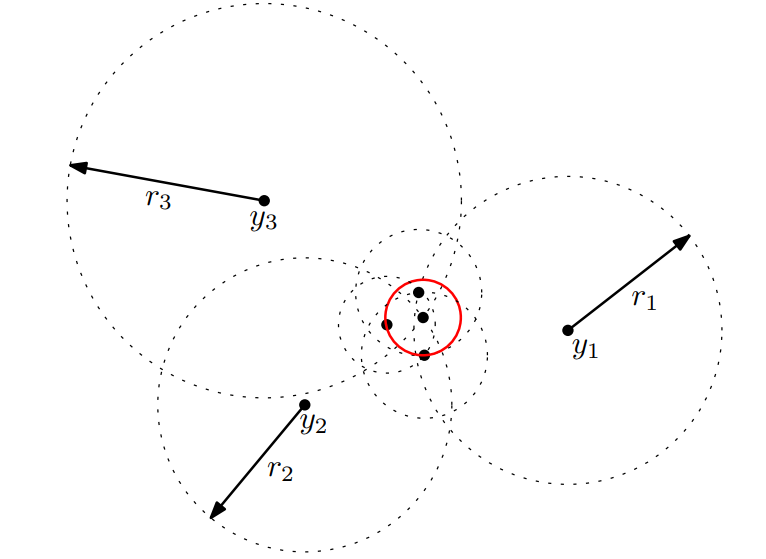
\includegraphics[width=5cm, height=4cm]{RDE.png}} 
\end{center}

\begin{theorem}
Точка $x_{i^*}$, возвращаемая алгоритмом RDE удовлетворяет условию
\[\mathds{P} (||x_{i^*} - x^*|| \le 3 \e) \ge 1 - e^{-\frac{m}{18}}\]
\end{theorem}

Пусть точки $x_i$ ($i = 1, ..., m$) таковы, что $\mathds{P} (f(x_i) - f^* \le \e ) \ge \frac{2}{3}$. Из $\mu$-сильной выпуклости следует, что $\mathds{P} (||x_i - x^*|| < \sqrt{\frac{2 \e}{\mu}} =: \delta) \ge \frac{2}{3}$. Применив к этим точкам алгоритм RDE, получим точку $x_{i^*}$, удовлетворяющую неравенству $\mathds{P}(||x_{i^*} - x^*|| < 3 \delta) \ge 1 - e^{-\frac{m}{18}}$. Из $L$-гладкости функции $f$ тогда следует, что $\mathds{P}(f(x_{i^*}) - f^* \le \frac{L}{2}(3\delta)^2 = 9 \frac{L}{\mu}\e) \ge 1 - e^{-\frac{m}{18}}$. Таким образом, генерируя точки алгоритмом, дающим гарантии сходимости с точностью $\e$ по матожиданию, но не с высокой вероятностью, мы предъявили алгоритм, дающий гарантию сходимости с высокой вероятностью, но лишь с $\kappa \e$-точностью, где число обусловленности $\kappa = \frac{L}{\mu} \gg 1$ может быть достаточно большим. Для нивелирования этой проблемы в статье \cite{davis2021low} был предложена процедура $proxBoost$.

\subsection{proxBoost}
Зафиксируем возрастающую последовательность $\lambda_0, ..., \lambda_T$ и последовательность точек $x_0, ..., x_T$. Для каждого $i = 0, ..., T$ введем функцию 
\[f^i(x):=f(x) + \frac{\lambda_i}{2}||x - x_i||^2\]
\[\bar{x}_{i + 1} := \argmin_x f^i (x)\]

В качестве $x_i$ можно брать $x_i = \bar{x}_i$ для $i \ge 1$. Так как точное вычисление точки минимума чаще всего невозможно, будем следить лишь за $||\bar{x}_i - x_i||$. Для простоты, $\bar{x}_0 := \argmin f$, $\lambda_{-1} := 0$.

\begin{theorem}
    (Inexact proximal point method) Для всех $j \ge 0$ выполняется следующее неравенство:
    \[f^j(\bar{x}_{j + 1}) - f^* \le \sum_{i = 0}^{j}\frac{\lambda_j}{2}||\bar{x}_i - x_i||^2.\]
    Слндовательно, имеем декомпозицию функциональной ошибки:
    \[f(x_{j + 1}) - f^* \le (f^j(x_{j + 1}) - f^j(\bar{x}_{j + 1})) + \sum_{i = 0}^{j}\frac{\lambda_j}{2}||\bar{x}_i - x_i||^2.\]
    Если функция $f$ еще и $L$-гладкая, то для всех $j \ge 0$ выполнена оценка:
    \[f(x_j) - f^* \le \frac{L + \lambda_{j - 1}}{2} ||\bar{x}_j - x_j||^2 + \sum_{i = 0}^{j - 1}\frac{\lambda_j}{2}||\bar{x}_i - x_i||^2.\]
\end{theorem}

Основным результатом Теоремы 2 является декомпозиция функциональной ошибки на ошибку на последнем шаге $(f^T(x_{j + 1}) - f^T(\bar{x}_{j + 1}))$ и накопленную ошибку $\sum_{i = 0}^{T}\frac{\lambda_j}{2}||\bar{x}_i - x_i||^2$. Для достаточно больших $T$ можно гарантировать то, что функция $f^T$ хорошо обусловлена. Использование результатов теорем 1 и 2 позволило авторам \cite{davis2021low} разработать алгоритм $proxBoost$.

\begin{algorithm}
            \caption{$proxBoost(\delta, p, T)$} \label{algorithm: cds bw}
            \textbf{Input:}
            $\delta \ge 0$, $p \in (0, 1)$, $T \in \mathbb{N}$
            \State Set $\lambda_{-1} = 0$, $\e_{-1} = \sqrt{\frac{2\delta}{\mu}}$
            \State Найти точку $x_0$ такую, что $||x_0 - \bar{x}_0|| \le \e_{-1}$ с вероятностью $1 - p$
            \hspace*{\algorithmicindent} 
            \begin{algorithmic}
                    \For{$j = 0, ..., T - 1$}
                    \State Set $\e_{j} = \sqrt{\frac{2\delta}{\mu + \lambda_j}}$
                    \State Найти точку $x_{j + 1}$ такую, что $\mathds{P}(||x_{j + 1} - \bar{x}_{j + 1}|| \le \e_{j}|E_j) \ge 1 - p$, где событие $E_j := \{x_i \in B_{\e_{i - 1}}(\bar{x}_i) \ \forall i \in [0, j]\}$
                    \EndFor   
                    \State Найти точку $x_{T + 1}$ такую, что $\mathds{P}(f^T(x_{T+1}) - \min f^T \le \delta |E_j) \ge 1 - p$   
            \end{algorithmic}
            \State \textbf{Output:} 
            $x_{T + 1}$
    \end{algorithm}
Алгоритм $proxBoost$ состоит из 3 шагов. На первом шаге ищется точка, довольно близкая к точке минимума функции $f$ с большой вероятностью. Эта задача может быть решена с помощью техники RDE. На втором шаге в цикле точно также можно решить аналогичные задачи для функциий $f^j$. На последнем шаге
\bibliographystyle{unsrtnat}
\bibliography{references}
\end{document}
